% !TeX spellcheck = en_US
\section{Superconductivity}

Superconductors have zero resistivity below a critical temperature $T_C$. 

\subsection{Meissner effect\buch{731}}
Superconductors expel magnetic fields from the bulk of the sample, which
is a perfectly diamagnetic behavior.
The superconductor develops a magnetization $M$ such that $M$ and the
applied field cancel everywhere.

\begin{figure}[ht!]
    \centering
    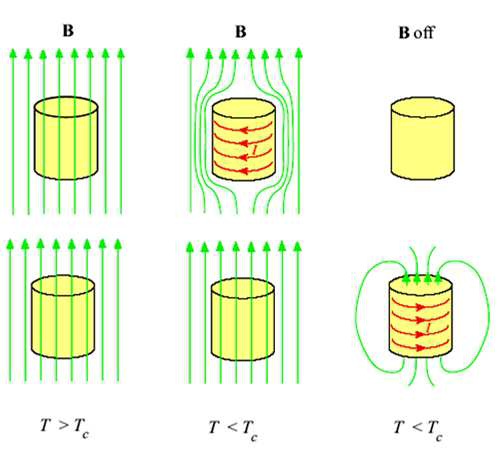
\includegraphics[width=0.4\linewidth]{images/superconductor.png}
    \caption{Magnetization inside a superconductor (above) and inside a perfect conductor (below)}
\end{figure}

Below $T_C$, a superconductor therefore has $\chi_m = -1$.

The magnetic field penetration is
\begin{equation}
    B(x) = B_0 e^{-\frac{c}{\lambda}}
\end{equation}
where $\lambda \approx \SIrange[range-phrase=\ldots]{10}{100}{\nano\meter}$ at $T=\SI{0}{\kelvin}$ is the penetration length.

\subsection{Type I and type II superconductors\buch{734}}
Type I superconductors have a sharp transition at $B_C$, while 
type II superconductors have no sharp transition.

\subsection{Critical current density\buch{736}}
Superconducting state is lost at current densities $>J_C$.
Thus there exists a critical surface in the $J,B,T$-space, for which a material is a superconductor.

\subsection{Superconductivity origin\buch{739}}
\subsubsection{Josephson effect\buch{756}}